\chapter{Background and Rationale}

\section{Background}

This project aims to create a serious game based on a robot in a remote laboratory. Moreover, it
aims to create a complete visual programming experience to teach the basics of programming. Thus,
in this state of the art, the three main topics that the project uses as a base will be covered and
deepened.

\subsection{Remote Laboratories}

Remote laboratories are usual laboratories, with the peculiarity that they can be accessed through
the Internet~\cite{remote_labs}. They give students the option to use the laboratory from home even
when the university or school is closed. This means that the students are able to do their homework
or experimentation using the equipment at their school or university without the need for them to be
physically there.

Currently they are becoming more popular due to the competitive advantage they can give to schools
and universities. Since there is no need for the student to be physically in the laboratory, the
laboratory does not need to be physically in the school or university, giving the option to share
laboratories between institutions and thus giving important economic benefits without reducing
the practice time of the students, or even increasing it.

Therefore, remote laboratories can be really helpful in teaching main concepts about science and
technology. The next laboratories are the most known ones that are working with science and
technology.

\subsubsection{Global Online Laboratory Consortium}

The \acrlong{golc} or \acrshort{golc} is an organization that focuses on the promotion of the
development of remote laboratories for educational use. They commonly promote remote laboratories
through conferences~\cite{golc1st}. They also support and encourage the sharing of these
laboratories between institutions.

\begin{figure}[!htbp]
	\centering
	
\includegraphics[width=0.35\textwidth]{fig/golc-award}
	\caption{\acrshort{golc} Online Laboratory Award 2015}\label{fig:golc_award}
\end{figure}

For promoting laboratories, they created an award (figure~\ref{fig:golc_award}) for remote
experimentation and another one for simulated experimentation.

\subsubsection{WebLab-Deusto}

WebLab-Deusto is a remote laboratory located at the University of Deusto, Bilbao. There are multiple
types of laboratories there, and all is being controlled by a software they developed, called
WebLab. Moreover, Pablo Orduña, one of it's main researches developed a complete federation model
to be able to share laboratories across the world~\cite{porduna_phd} transparently to the final
user.

In WebLab-Deusto they created one of the most used remote laboratories in electronics teaching. It
is called \acrlong{visir} or \acrshort{visir}~\cite{visir}, and it recreates electronic circuits
made visually by students in real hardware so that students can take real measurements.

\begin{figure}[!htbp]
	\centering
	
\includegraphics[width=0.35\textwidth]{fig/weblab}
	\caption{WebLab-Deusto logo.}
\end{figure}

\subsubsection{\acrshort{golab} Project}

The \acrshort{golab} Project, or \acrlong{golab} uses remote and virtual laboratories to encourage
young people from 10 to 18 years old to learn about \acrlong{stem}
(\acrshort{stem})~\cite{golab_web}. They have created a web portal to access those laboratories.
They collaborate with many remote laboratories, such as WebLab-Deusto, for instance.

\begin{figure}[!htbp]
	\centering
	
\includegraphics[width=0.25\textwidth]{fig/golab}
	\caption{\acrshort{golab} Project logo.}
\end{figure}

\subsubsection{iLab Project at \acrshort{mit}}

The \acrlong{mit} has its own remote laboratory platform called iLab. They have many remote
laboratories where they experiment with \acrlong{dsa}s (\acrshort{dsa}), heat exchangers and even
with polymer crystallization. It has even inspired some big projects using this technology such as
an on-line repository to locate remote laboratories~\cite{ilabs_multi}.

\begin{figure}[!htbp]
	\centering
	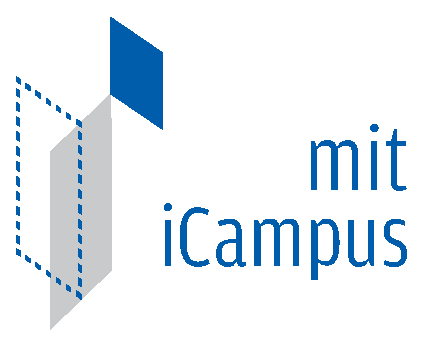
\includegraphics[width=0.35\textwidth]{fig/icampus.eps}
	\caption{iCampus logo, project at \acrshort{mit} where iLabs have been created.}
\end{figure}

This project is part of the iCampus project~\cite{icampus_web}, a project that started in 1999 as a
research alliance between \acrshort{mit} and Microsoft Research. They develop and sponsor innovative
projects in \acrshort{mit} and elsewhere.

\subsubsection{Robotic remote experiments}

Some of the laboratories listed before have currently implementations of robotic experiments as a
teaching material in some areas. In WebLab-Deusto, for example, they have what they call WebLab-Bot
(figure~\ref{fig:weblab-bot}). This robot is based on Azkar-Bot~\cite{azkar_bot} robot and it is
used for electronic students to learn how to program it. They have simple demonstrations that follow
a black line or respond to simple commands.

\begin{figure}[ht]
	\centering
	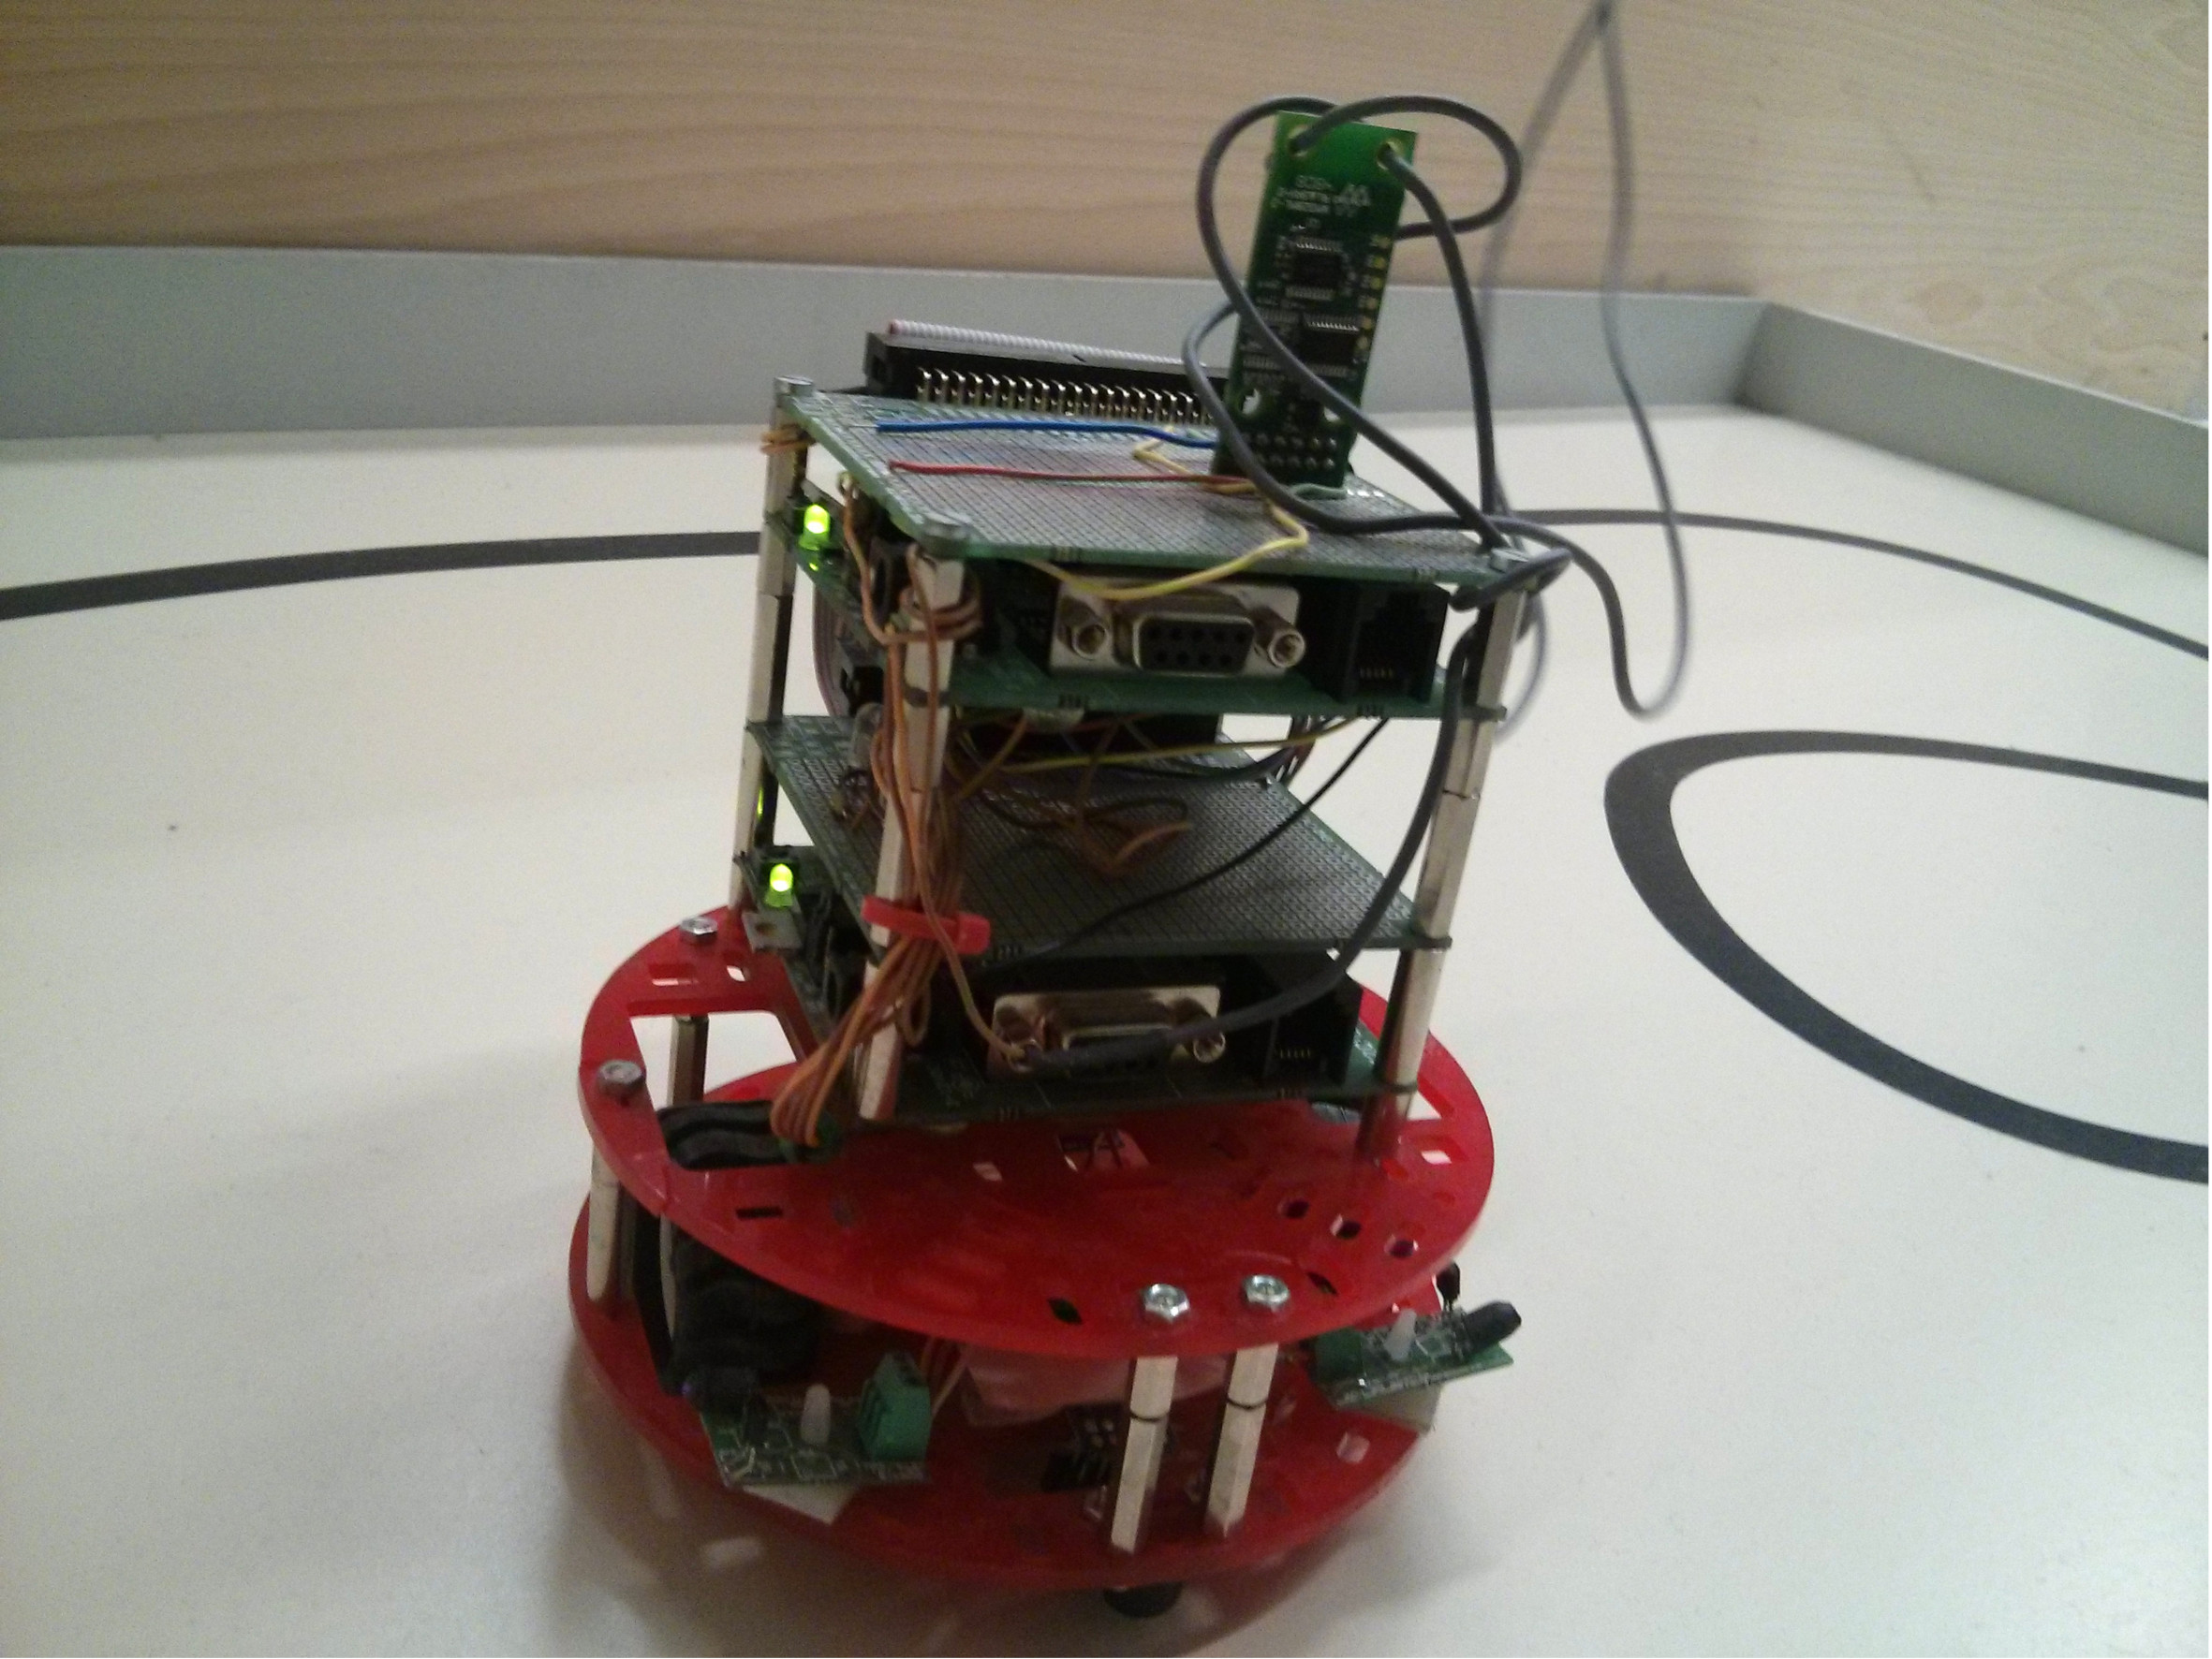
\includegraphics[width=0.5\textwidth]{fig/weblab-bot.jpg}
	\caption{WebLab-Bot, a robot based on Azkar-Bot. A remote laboratory in WebLab-Deusto.}
	\label{fig:weblab-bot}
\end{figure}

Moreover, in \acrlong{tli} (\acrshort{tli}), they have a robot called iRobot, that teaches how to
deal with accuracy of sensors, localization and mapping. Finally, the robot that will be used in
this project is called Romie (Figure~\ref{subfig:romie}). It is located in WebLab-Deusto and it has
the needed functionality for this project: it is capable of following a line, it detects walls and
intersections. WebLab-Deusto has a complete labyrinth for it where this project will be deployed
(figure~\ref{subfig:labyrinth}).

\begin{figure}[ht]
	\centering
	\begin{subfigure}{0.35\textwidth}
		\centering
		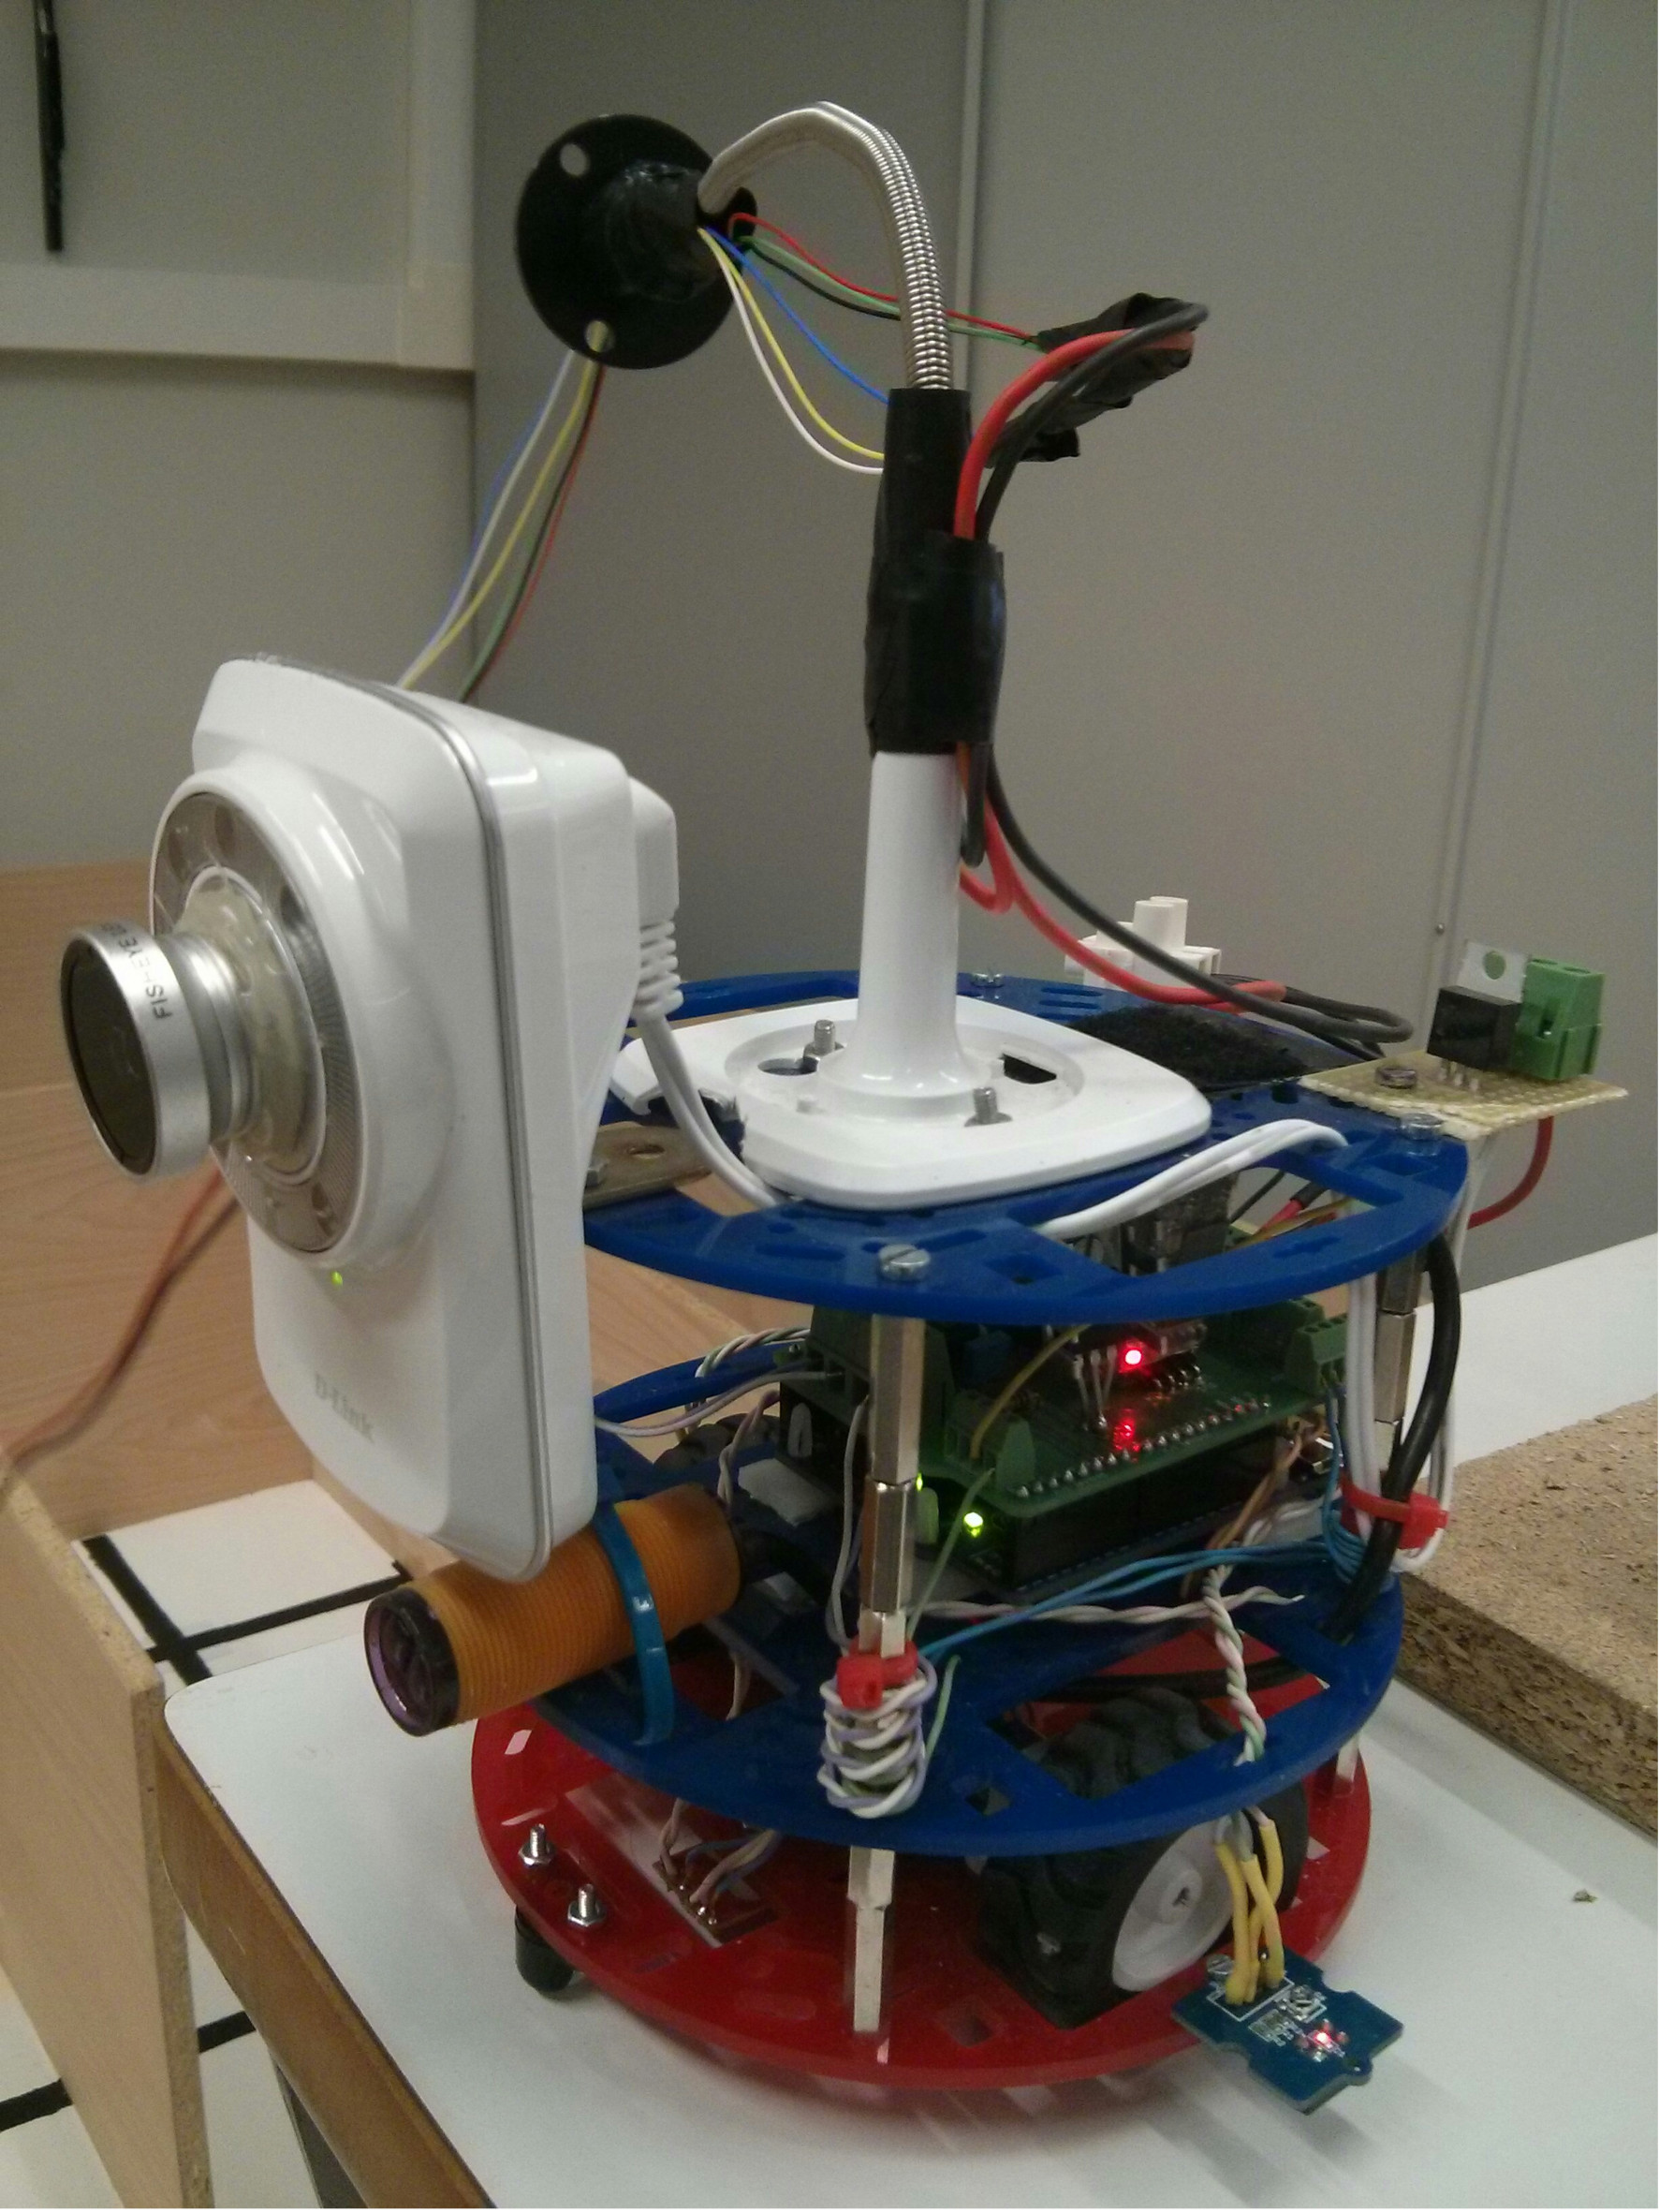
\includegraphics[width=0.8\textwidth]{fig/romie.jpg}
		\caption{Romie, the robot.}\label{subfig:romie}
	\end{subfigure}\quad
	\begin{subfigure}{0.55\textwidth}
		\centering
		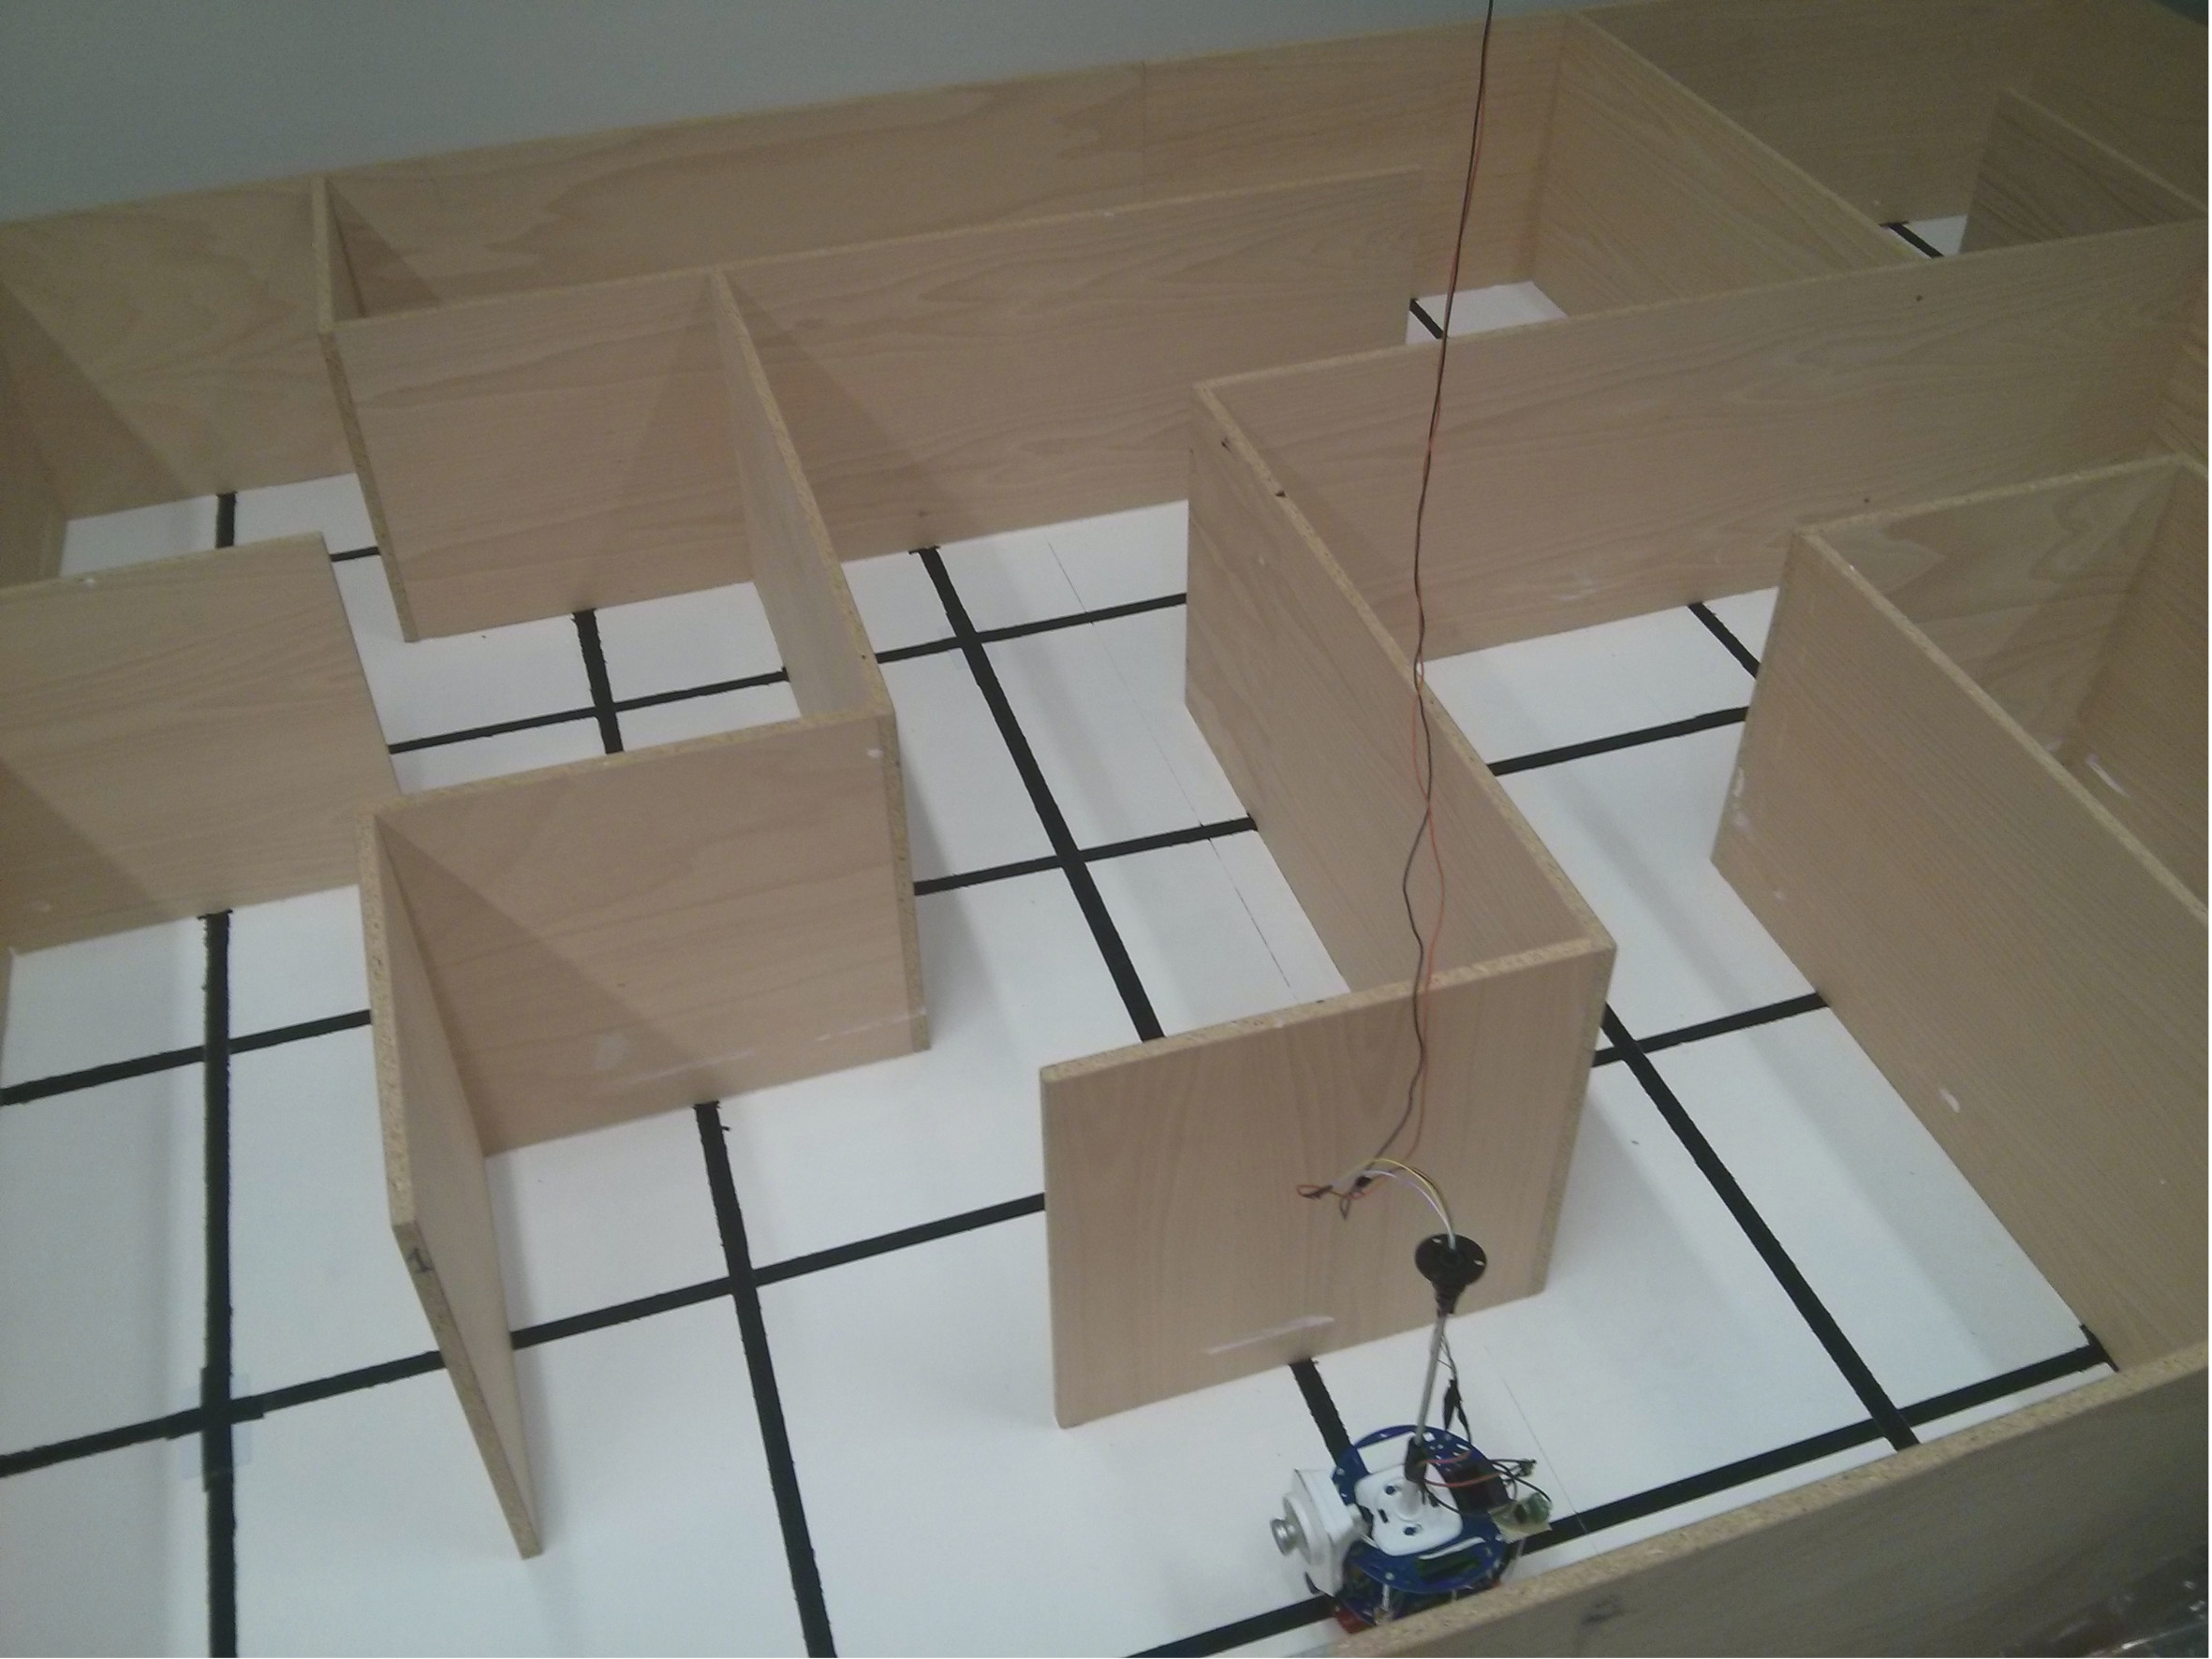
\includegraphics[width=0.8\textwidth]{fig/labyrinth.jpg}
		\caption{The labyrinth where Romie will have to move.}\label{subfig:labyrinth}
	\end{subfigure}\quad
	\caption{The robot that will be used in this project.}
\end{figure}

\subsubsection{Simulations}

Even if the project will not be based on simulated robotics but in real robots, currently some
projects use simulations to bring some of the experience to users. A simulation is usually less
costly than a remote laboratory, since not much specialized hardware is required. On the other hand,
students will not be using real tools and experimentation environments, so the experience of using
them will not be as complete as in a remote laboratory.

Nevertheless, some prefer creating hybrid laboratories~\cite{hybrid_labs}. In these cases, the
laboratories add a simulation layer over the real laboratory. This way, the user still uses a real
laboratory, with the benefits of knowing how to use the laboratory and doing real experimentation,
and it also gives the user some more benefit by simulating extra conditions that could be expensive
to create in a real laboratory.

\subsection{Serious Games and Visual Programming}

Serious games are video games that do not only entertain, but they manage to teach. Thanks to that,
they can be used to improve the quality of the learning environment for students. Moreover, since
games in many cases attract better the attention of young people, they can even be a better tool for
teaching, at least, the basic concepts of some subjects~\cite{serious_games}. Now the most known
tools for visual programming environments will be analyzed, since these tools will be the ones used
for creating one of the scenarios.


Visual programming is a way of programming that instead of using real code in a real programming
language uses a visual interface to create programs and then translate them to a well known
language. This way, people that are not yet used to programming languages, interfaces such as
\acrshort{ide}s (\acrlong{ide}s) or code execution, and do not understand the basis of programming
can start learning by using a simple visual environment~\cite{visual_programming}.

\subsubsection{Scratch}

Scratch is one of the most known visual programming tools~\cite{scratch}. It is in itself an
\acrshort{ide}, made by the \acrshort{mit} to help to teach programming to inexperienced users. It
teaches the basic concepts of algorithms and it gives an enough powerful tool so that users can
enjoy using it. It's main concept is to join basic programming blocks so that functionality is
created.

Moreover, they have created a complete collaboration platform where all the users of Scratch can
share their creations and check out the ones that others have made. That way, users can learn more
by looking at code created by others.

\subsubsection{Blockly}

Blockly, unlike Scratch, is not a visual programming \acrshort{ide}, but a visual programming
library to create visual programming editors and \acrshort{ide}s. It has the same basis as Scratch,
so it contains basic programming blocks to build applications by joining them
(Figure~\ref{fig:blockly}), and it also gives developers the option to create their own blocks with
a simple \acrlong{api} or \acrshort{api}. It was created by Google and it's source is now available
in GitHub~\cite{blockly}.

\begin{figure}[ht]
	\centering
	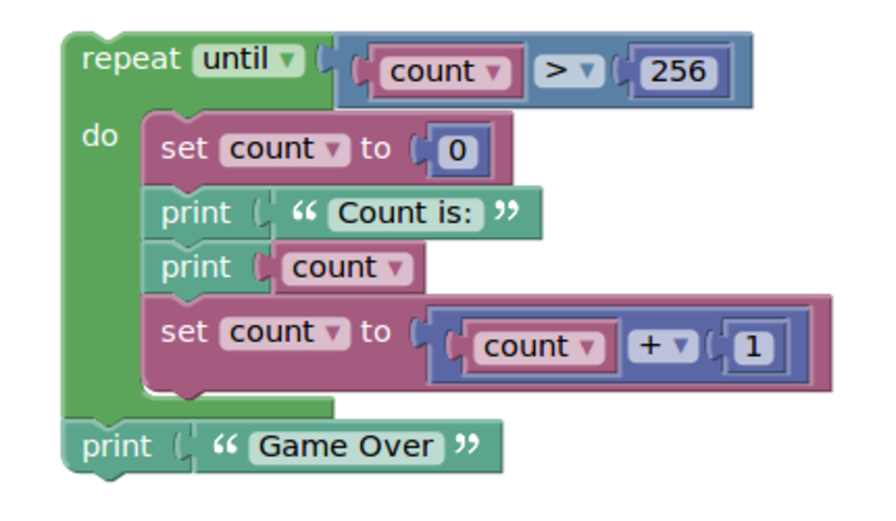
\includegraphics[width=0.5\textwidth]{fig/blockly}
	\caption{Simple program example created in Google's Blockly.}\label{fig:blockly}
\end{figure}

Blockly enables developers to create their own programming environments for their projects, so they
can adapt Blockly itself to their needs, and thus, making it possible for them to even create
complete \acrshort{ide}s for their projects based on visual programming.

\subsection{WebLab-Deusto}

WebLab-Deusto is a remote laboratory facility located in the University of Deusto, Bilbao. Since
2001, it has been providing students with remote laboratories to complete their academic
learnings~\cite{weblab}. Since then, it has been extended and many of it's laboratories is available
all over the world. It's no longer a laboratory only made for microelectronics university students
since nowadays it serves schools and universities everywhere to provide them with remote
laboratories.

Among others, it serves an experiment to prove and measure the Archimedes' principle
(Figure~\ref{fig:archimedes}), an experiment to program and control a robot and some
microelectronics experiments with \acrlong{pld}s or \acrshort{pld}s and \acrlong{fpga}s or
\acrshort{fpga}s. Moreover, there are more laboratories in development, such as an elevator to teach
students how to program and control them, an experiment with an aquarium where students can feed
them and, of course, the project presented here: a complete learning and gaming experience brought
remotely using a robot, Romie.

\begin{figure}[!htbp]
	\centering
	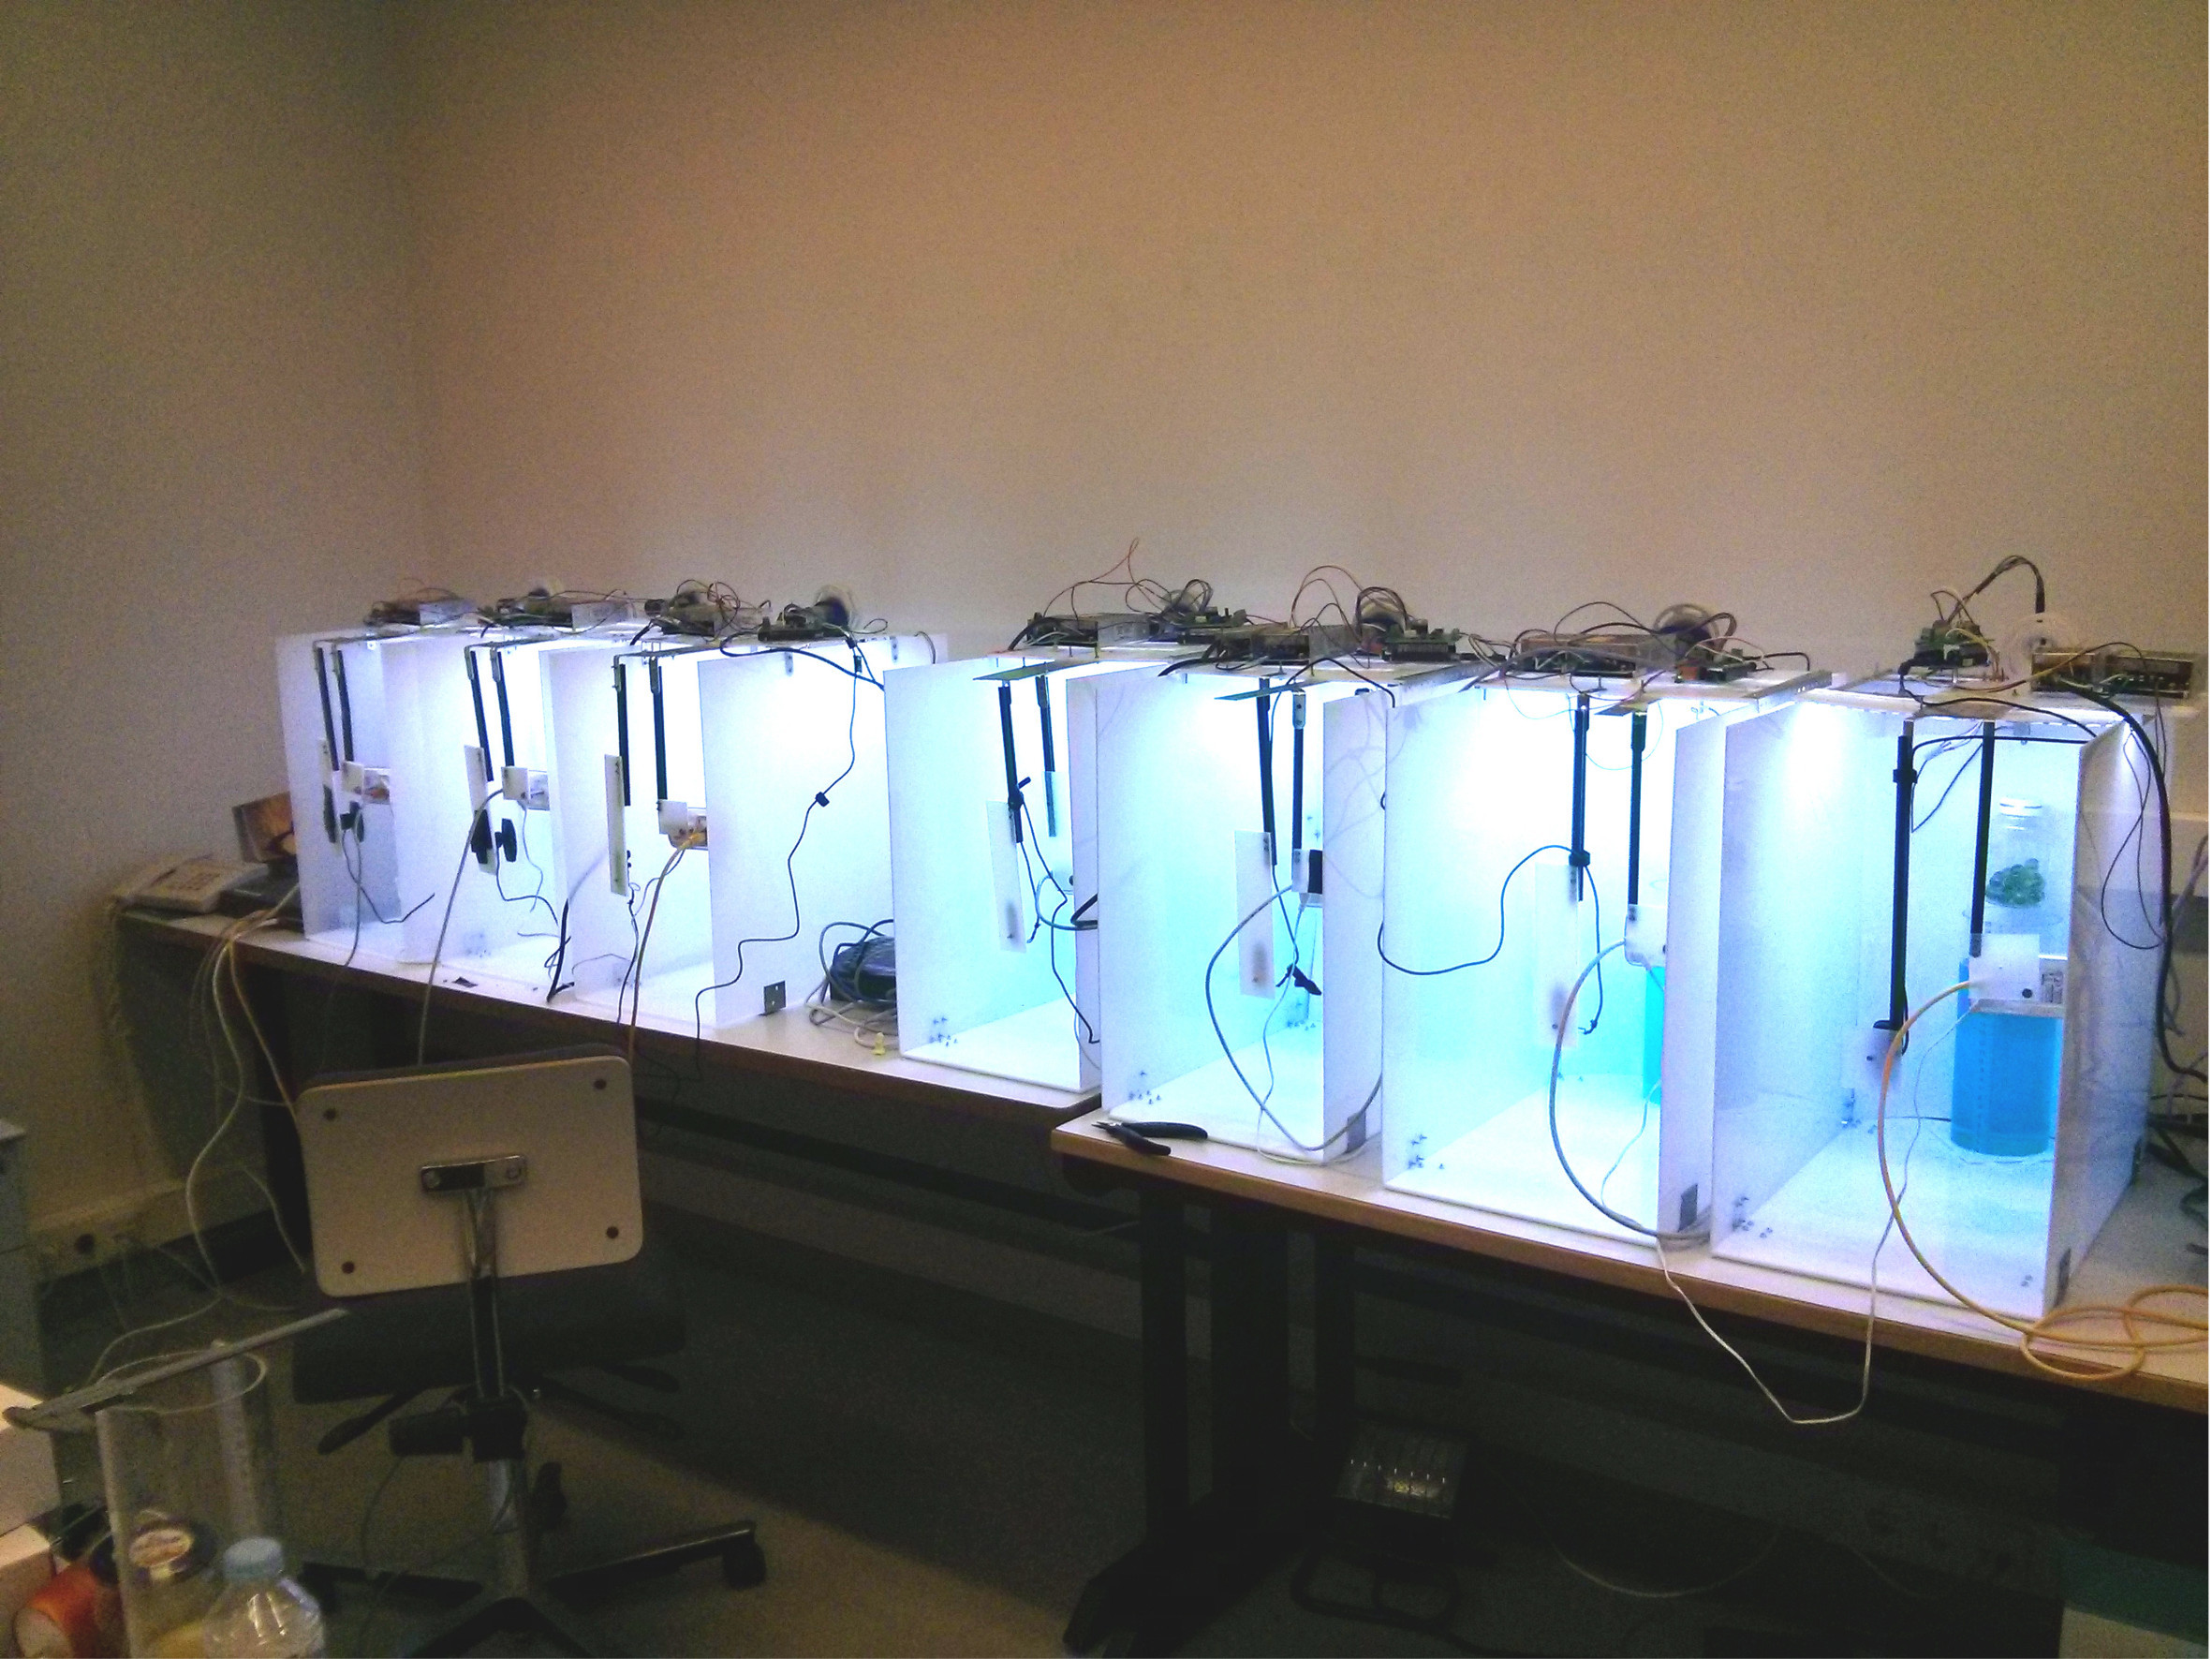
\includegraphics[width=0.5\textwidth]{fig/archimedes.jpg}
	\caption{Archimedes experiment in WebLab-Deusto.}\label{fig:archimedes}
\end{figure}

\section{Rationale}

Remote laboratories are a platform developed to reduce costs of experimentation for schools by
moving the laboratories themselves to the cloud. Nevertheless, this is only one of the multiple uses
a platform like this can have, and in this project, the challenge is to demonstrate how remote
laboratories can be used for serious gaming.

This project will be to the best of the knowledge provided by this research the first game platform
based on remote laboratories, it will open the course to future developments in this area by
enabling future games to be developed using this technology.

It will be a challenge to adapt the current technology and experimentation platforms to this kind of
project, but the result can be unique and powerful for teaching all kind of knowledge in a fun way
by using real gamification processes in a remote laboratory platform.
